\documentclass[9pt,twocolumn]{article}

\usepackage{amsmath,amssymb,enumerate,algorithm,algorithmic,fullpage,graphicx}

\usepackage{setspace}

\setlength{\columnsep}{1cm}
\everymath{\displaystyle}

\usepackage{titling}
\newcommand{\subtitle}[1]{%
  \posttitle{%
    \par\end{center}
    \begin{center}\large#1\end{center}
    \vskip0.5em}%
}

\title{Applying Varied Artificial Intelligence Techniques to Play 2048}
\subtitle{CS 221 Project Report}
\author{Zhiyang He, Charles Lu, Stephen Ou \\ \texttt{\{hzyjerry,clu8,sdou\}@stanford.edu}}
\date{December 11th, 2015}

\begin{document}

\maketitle

\section{Introduction}

Released in 2014, the single-player puzzle game 2048 quickly became a worldwide sensation: in addition to hijacking classrooms and quickly occupying people's phone screens, it also spawned countless spin-offs, strategy guides, and self-professed gurus. Meanwhile, the game offers a good platform to experiment and compare both traditional and cutting edge artificial intelligence techniques.

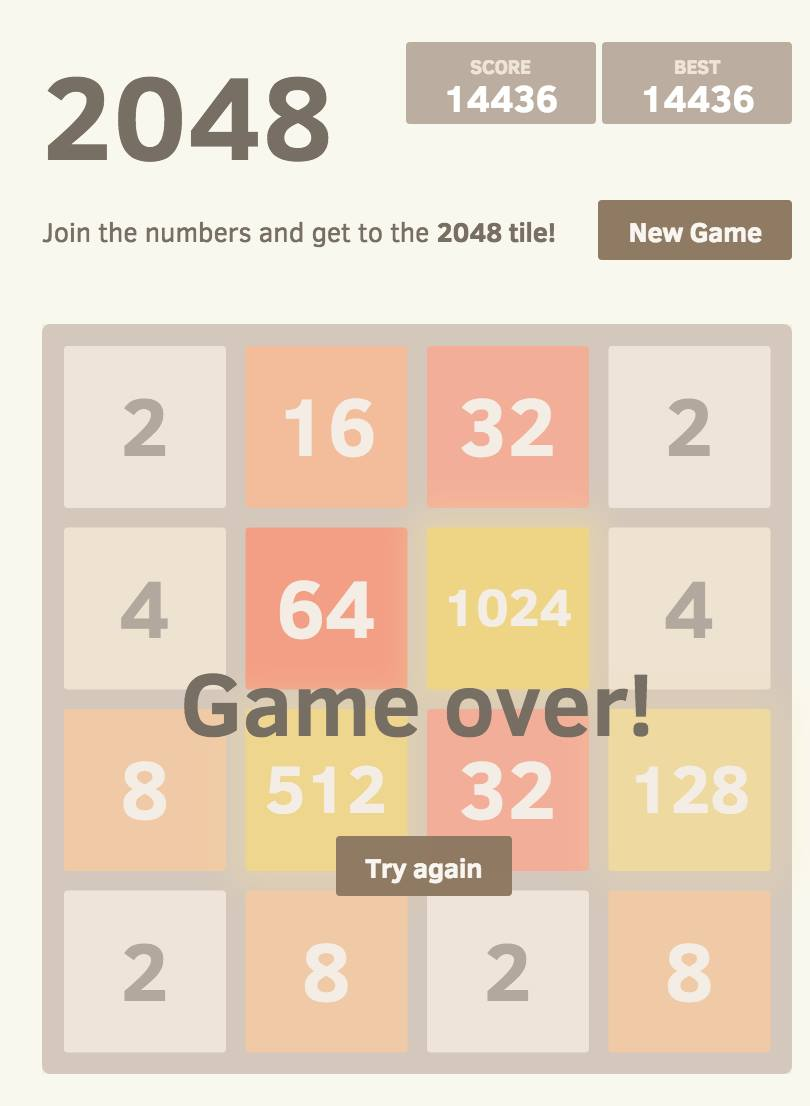
\includegraphics[width=60mm]{2048_screenshot2.jpg}

2048 is played on a 4 by 4 grid. Every turn, a random tile with a value 2 or 4 will appear on an empty cell. Then the player can choose to slide left, right, up, or down. All the tiles will slide all the way towards that direction. If any two tiles collide and have the same value, they will merge into one tile, with a new value being the sum of the two old tiles. Additionally, when two tiles collide, the score will be incremented by the value of the newly merged title. There are two ways to end the game. If the value of one tile reaches 2048, the game is considered a win (though the player can continue playing). Otherwise, if all the cells on the grid are occupied with mismatched tiles and no move is possible, the game is lost.

\section{Literature Review}

Since its release, many AIs have been built to play 2048. All implementations we have seen use some form of searching the game tree.

One of the most widely known 2048 AIs was published by Matt Overlan, who used an algorithm with iterative deepening depth-first alpha-beta search.[1] The evaluation function tries to keep the rows and columns monotonic (either all decreasing or increasing) while aligning same-valued tiles and minimizing the number of tiles on the grid.

2048 was also the topic of choice for three projects in 2014's CS 221 class.[2][3][4] All three projects explored only search techniques, e.g. expectimax, and also explored optimization and pruning methods to improve computation time.

\section{Task Definition}

Our goal for this project is to build and investigate a number of models which play to maximize the game score at a reasonable runtime. The input-output behavior is as follows: on each turn, given the state of the 2048 game board (as well as move history when necessary), our models will return one of four moves (left, right, up, down) to attempt to maximize the score.

The game of 2048 can be modeled using a series of game states, encoding the status of the 16 squares on the board. The board is represented as a 2 dimensional list of integers, each cell containing a power of 2 representing the current value of that cell. 0 is used to indicate unoccupied cells. The score variable is used to keep track of all the points received so far. The rule of the game of 2048 states that score is incremented by the sum of the two tiles when two tiles with the same value get merged.

To facilitate the state-based model, we also implement two main methods that are available through the 2048 game state: \texttt{getLegalActions()} and \texttt{generateSuccessor()}:

\texttt{getLegalActions()}: If the current agent is the human, there are four possible moves. The human can swipe left, right, up, or down. There is one special case. A move is considered invalid if the board in the successor state is the same as the current state. For example, if the left three columns are all filled with tiles and they are have different values, swiping left is not a valid action because the successor state will not change. If the current agent is the computer, there are maximum of sixteen possible moves. The computer can add a new tile with a value of 2 into an unoccupied cell.

\texttt{generateSuccessor()}: If the current agent is the human, all the tiles will slide in the direction specified. If two neighboring tiles in that direction have the same value, they will collide and form a new tile with a new value that is the sum of the two old values. For example, consider a board with only two tiles, both with a value of 2, on the bottom row. Swiping left will result in a merged tile with a value of 4, sitting in the bottom left corner. (See \texttt{gameState.py} for more complex merging behaviors.) Next, if the current agent is the computer, a new tile with the value of 2 will be added at the specified cell given by the row and column number.

In order to maximize the game score of 2048, we first built six agents, three of which are baseline algorithms and three of which are more advanced search algorithms that we learned in class. We then used the results from these six agents to train reflex-based models, and also explored reinforcement learning-based models.

\begin{enumerate}[1)]

\item \textbf{Random agent.} This baseline agent simply picks a random move.

\item \textbf{Up down agent.} This baseline agent alternates between moving up and down.

\item \textbf{Up left agent.} This baseline agent alternates between moving up and left.

\item \textbf{Expectimax agent.} This agent searches the expectimax game tree to a given depth and returns the maximizing move.

\item \textbf{Minimax agent.} This agent searches the minimax game tree to a given depth and returns the maximizing move.

\item \textbf{Minimax agent with alpha-beta pruning.} This agent returns the same results as the minimax agent, but uses alpha-beta pruning to improve computation efficiency.

\end{enumerate}

For the expectimax, minimax, and alpha-beta pruning agents, which require a way to score the current game state, we experimented with a number of evaluation functions. Though the purpose of this project was not to find the ideal evaluation function or tune perfect hyperparameters for our evaluation functions, the best evaluation function we used with the expectimax agent (with a depth of 3) had a win rate of 100 percent (getting to 2048 on every game).

Though the expectimax agent yielded very good results, the main disadvantage of using it was its computation time. With a branching factor of up to 4 for the player’s move and up to 16 for the computer’s move (placing an empty tile), it is quite infeasible to search the game tree to a large depth without pruning. Specifically, on a modern laptop, it took the expectimax agent with depth 3 almost a second per move.

Therefore, we next attempted to use the “optimal” moves suggested by the expectimax agent to train various reflex models using different machine learning techniques. Specifically, to generate the training, validation, and test datasets, we simply ran multiple playthroughs of 2048 using the search agent, and saved each game board state and the corresponding recommended move as a single data point.

Finally, we approached the game with a reinforcement learning strategy using Q-learning, which has not previously been applied to playing 2048 in a publication. Inspired by DeepMind's deep Q-learning strategy for playing Atari games,[5] we applied a similar approach to tackle the 2048 puzzle, using Q-learning with a neural network. This strategy has the advantage of being model-free, and thus needing no prior knowledge of the game.

\section{Infrastructure}

The primary infrastructure for modeling the game state and logic and implementing the AI agents was implemented in Python. For a more human-friendly user interface, we also built a front end web interface to play the game and visualize the AI agents' moves. We forked the original 2048 repository by Gabriele Cirulli and added our custom Javascript functions which communicate with a lightweight Python server which computes the optimal move. The setup used Flask,[6] an open source Python web framework. We wrote a JavaScript function that serializes the current board as a string and passes it to the Flask server via an AJAX request. The server computes the optimal move using a specified approach, and returns a response back to the front end. Then, a callback JavaScript function updates the board using the optimal move.

One problem we ran into while doing simulation is that the HTTP request and overhead of displaying the front end visualization was a bottleneck in terms of speed. While it is interesting to see the game being solved in the real user interface, the speed becomes problematic when we wanted to do a lot of simulation to get abundant results. Therefore, we built a more robust back end simulator which runs the game from the command line. Without involving the front end, the back end-only simulator is able to finish one full game in just a few seconds.

To further increase the speed of the simulation, we decided to take advantage of Stanford's computing resources. We parallelized the game simulation across 30 myth machines and ran them concurrently to get results. We were able to run 100 full iterations of the game across all 30 machines in less than one minute.

\section{Approaches}

We applied several different agents to the 2048 game, each using a different technique---either a strategy specific to 2048, a search strategy using the game tree, a reflex strategy, or a reinforcement learning strategy.

For each strategy, we simulated the game 300 times and recorded their scores and other statistics.

\subsection{Basic Strategies}

The first agent that we implemented was a random agent that simply picks a random move without considering the game state. This is meant to serve as a baseline.

\begin{table}[!htbp]

\centering

\begin{tabular}{|l|l|}
\hline
Mininum Score      & 140 \\ \hline
Maximum Score      & 1456 \\ \hline
Mean Score         & 571.255 \\ \hline
Median Score       & 546 \\ \hline
Standard Deviation & 280.527 \\ \hline
\end{tabular}

\caption{Random Agent}

\end{table}

The up down agent alternates between moving up and down. This method simulates a player who does not play randomly and simply swipes up and down.

\begin{table}[!htbp]

\centering

\begin{tabular}{|l|l|}
\hline
Mininum Score      & 64 \\ \hline
Maximum Score      & 156 \\ \hline
Mean Score         & 94.775 \\ \hline
Median Score       & 88 \\ \hline
Standard Deviation & 18.791 \\ \hline
\end{tabular}

\caption{Up Down Agent}

\end{table}

The up left agent alternates between moving up and left. This method is employed as a strategy by many novice players to obtain relatively high scores. This is meant to trap the highest value tile towards the top left corner and make it easier to coalesce similar valued tiles.

\begin{table}[!htbp]

\centering

\begin{tabular}{|l|l|}
\hline
Mininum Score      & 656 \\ \hline
Maximum Score      & 1708 \\ \hline
Mean Score         & 946.457 \\ \hline
Median Score       & 796 \\ \hline
Standard Deviation & 261.353 \\ \hline
\end{tabular}

\caption{Up Left Agent}

\end{table}

\subsection{Search Strategies}

We then implemented more advanced strategies which traverse the game tree using expectimax, minimax, and minimax with alpha-beta pruning. In the normal game of 2048, the computer move (where the new tile is inserted) is randomized, so technically only the expectimax strategy makes sense in that environment. However, we wanted to experiment with minimax strategy as well to see how the score differs if the AI agent assumes that the computer aims to minimize the player’s score when inserting a new tile.

Because of the number of path to explore in the game state is huge, our initial experimentation used a depth of 2. In addition to simply using the game score, we implemented several evaluation functions to provide an accurate estimate of how “good” a game board is:

\begin{enumerate}

\item \textbf{Game score evaluation function.} This evaluation function looks at the current score of the board and uses that to determine the value of the board.
\item \textbf{Empty tiles evaluation function.} This evaluation function simply counts the number of empty tiles on the board; more is better.
\item \textbf{Monotonicity evaluation function.} This evaluation function measures how much the rows and columns are sorted in increasing or descending order. Specifically, we count the total number of times the rows and columns switch from increasing to decreasing or vice versa. Smaller is better, so we take its reciprocal.
\item \textbf{Smoothness evaluation function.} This evaluation function sums the difference between each pair of adjacent tiles. Again, smaller is better so we take its reciprocal.
\item \textbf{Snake evaluation function.}[3] This evaluation function values tiles on the top left corner and devalues tiles on the bottom right corner in a snake shape. In effect, this organizes tile values with the highest value tiles positioned in the top left.

\end{enumerate}

We use a similar version of the expectimax algorithm as the one presented in lecture. If the current agent is the human, we take the action that produces the maximum score from the recursion tree. If the current agent is the computer, we randomly pick one action (to be more specific, an unoccupied cell location).

Overall, the snake evaluation function is especially successful, while the empty tile, monotonicity, and smoothness evaluation functions are not very useful when used alone.

\begin{table}[!htbp]

\centering

\begin{tabular}{|l|l|}
\hline
Mininum Score      & 5580 \\ \hline
Maximum Score      & 33900 \\ \hline
Mean Score         & 20293.433 \\ \hline
Median Score       & 20712 \\ \hline
Standard Deviation & 2956.264 \\ \hline
\end{tabular}

\caption{Expectimax Agent with depth 2 and snake evaluation function}

\end{table}

\begin{table}[!htbp]

\centering

\begin{tabular}{|l|l|}
\hline
Mininum Score      & 1496 \\ \hline
Maximum Score      & 16364 \\ \hline
Mean Score         & 7397.181 \\ \hline
Median Score       & 7168 \\ \hline
Standard Deviation & 3250.412 \\ \hline
\end{tabular}

\caption{Expectimax Agent with depth 2 and game score evaluation function}

\end{table}

The monotonicity and smoothness evaluation functions unfortunately did not give an accurate estimate of the board, as the mean score hovers around 390 for both of them.

When using the snake evaluation function, we received astonishing results once we increased the depth to 3. This resulted in the \textbf{best} results out of all the agent, depth, and evaluation function combinations we tested which had reasonable running time.

\begin{table}[!htbp]

\centering

\begin{tabular}{|l|l|}
\hline
Mininum Score      & 81900 \\ \hline
Maximum Score      & 172426 \\ \hline
Mean Score         & 137770 \\ \hline
Median Score       & 158984 \\ \hline
Standard Deviation & 48849.407 \\ \hline
\end{tabular}

\caption{Expectimax Agent with depth 3 and snake evaluation function}

\end{table}

This result makes sense because by considering an extra level, the agent has $4 \cdot 16 = 64$ times more game states to pick an optimal move from. This enables a more intelligent choice which was be able to increase our mean score significantly.

As mentioned above, even though the minimax algorithm does not fit the game perfectly because in the real 2048 game the computer picks a move random, we still attempted to validate the assertion that the score generated by the minimax agent is lower than that of the expectimax agent with the same depth and evaluation function. Our assumption is correct.

We use a similar version of the minimax algorithm as the one presented in lecture. If the current agent is the human, we take the action that produces the maximum score in the recursion tree. If the current agent is the computer, we take the action (considering all possible insertions of new tiles) with the minimum score in the recursion tree.

\begin{table}[!htbp]

\centering

\begin{tabular}{|l|l|}
\hline
Mininum Score      & 2600 \\ \hline
Maximum Score      & 21036 \\ \hline
Mean Score         & 13943.141 \\ \hline
Median Score       & 14804 \\ \hline
Standard Deviation & 5279.458 \\ \hline
\end{tabular}

\caption{Minimax Agent with depth 2 and snake evaluation function}

\end{table}

We use a similar version of the alpha-beta pruning algorithm as the one presented in lecture. It performs the same search as the minimax agent. However, if at any point as we loop through all the player's actions, the beta value is smaller or equal to the alpha value, we can terminate and return the maximum action so far. Similarly, on the computer's turn, if at any point as we loop through all the actions the beta value is smaller or equal to the alpha value, we can terminate and return the minimum action so far.

\begin{table}[!htbp]

\centering

\begin{tabular}{|l|l|}
\hline
Mininum Score      & 2368 \\ \hline
Maximum Score      & 24676 \\ \hline
Mean Score         & 15064.333 \\ \hline
Median Score       & 15660 \\ \hline
Standard Deviation & 4782.109 \\ \hline
\end{tabular}

\caption{Minimax with Alpha-Beta Pruning Agent with depth 2 and snake evaluation function}

\end{table}

\subsection{Reflex Strategies}

However, as mentioned above, the computation required for a depth of 3 is quite high, taking up to one second for each move. Therefore, as summarized above, we used training data from the expectimax agent’s moves to train various reflex models in Theano and Torch. We had a total of over 20,000 data points (consisting of a input in $\mathbb{R}^{16}$ and a move label corresponding to left, up, right, down).

We first implemented and trained a multi-class logistic regression model in Theano. In essence, we trained four logistic regressions (one for each move) with the entire dataset, corresponding to labels of 0 or 1 depending on whether the move was recommended or not. During prediction, we simply fed the board state into each model and went with the move with the highest expected “probability,” or the next highest scoring move if the top move was invalid.

\begin{table}[!htbp]

\centering

\begin{tabular}{|l|l|}
\hline
Mininum Score      & 320 \\ \hline
Maximum Score      & 400 \\ \hline
Mean Score         & 375.2 \\ \hline
Median Score       & 382 \\ \hline
Standard Deviation & 23.61 \\ \hline
\end{tabular}

\caption{Logistic regression classifier with no feature transform (raw tile value features)}

\end{table}

As demonstrated by the poor scores (even worse than random!), even with validation during training, the practical test error rate was very high.

The same technique was tried, but using the softmax function $\sigma(\mathbf{z})_j = \frac{e^{z_j}}{\sum_{k=1}^K e^{z_k}} \text{ for } j = 1, \dots, K$ [8], yielding similar results.

Noticing that the inputs (tiles on the game board) were all powers of two, we considered applying a simple feature transformation: taking the base-2 logarithms of all features. However, this actually worsened the prediction results:

\begin{table}[!htbp]

\centering

\begin{tabular}{|l|l|}
\hline
Mininum Score      & 268 \\ \hline
Maximum Score      & 272 \\ \hline
Mean Score         & 270.4 \\ \hline
Median Score       & 270.4 \\ \hline
Standard Deviation & 23.61 \\ \hline
\end{tabular}

\caption{Logistic regression classifier with feature transform (raw tile value features)}

\end{table}

Specifically, with a single-layer multi-class classifier using logistic regression, using the feature transform resulted in the predicted moves to always be “up”---again, likely a result of dataset bias as well as nonlinearity.

The above results are obviously very poor, but make sense given the hypothesized nonlinearity of the problem. Therefore, we next constructed various neural network models using Torch [7] with the same 16 inputs and 4 outputs, but an additional layer with a variable number of neurons. As with before, sigmoids were used in the first transformation and a softmax for the outputs. However, for all models, regardless of the size of the hidden layer, the model again failed to generalize and outputted similar prediction results as above.

\subsection{Reinforcement Strategies}

For the deep Q-learning strategy, our goal was to obtain an agent that maximizes the accumulative future reward. This feature is described by optimal Q-value $$Q^*(s, a) = \max_{\pi} \mathbb{E} [r_t + \gamma r_{t + 1} + \gamma r_{t + 2} + \dots | s_t = s, a_t = a, \pi]$$ which describes the maximum sum of rewards discounted by $\gamma$ at future steps t, achieved by a policy $\pi(s|a)$ after making an observation ($s$) and making an action ($a$). The Q-value (action-value) contains all pertinent information about the playing field along with a possible action. The Q-function (utility function) is used to describe how well our Q values approximates the actual game utilities: $$\hat Q_{\text{opt}(s, a)} \leftarrow (1-\eta) \underbrace{\hat Q_{\text{opt}(s, a)}}_\text{prediction} + \eta \underbrace{(r + \gamma \hat V_{\text{opt}(s')})}_\text{target}]$$

In the Q-learning algorithm, action utilities are evaluated based on immediate reward gained from taking actions, with the possibility of a delayed reward led to by the action. Due to the large state space of 2048 puzzle, our data cannot possibly exploit all the possibilities. Thus we use a Q-value outputted by neural network:

\begin{centering}

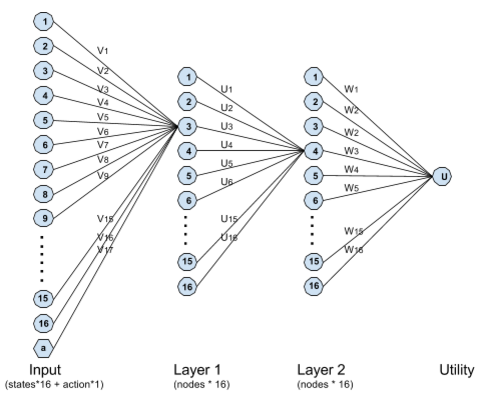
\includegraphics[width=60mm]{rl_nodes.png}

\end{centering}

By linking our trainer with reinforcement learning code using \texttt{popen()}, \texttt{write()}, and \texttt{read()} in Python, we apply real-time reinforcement learning to our game playing. Every time a game state is generated, we feed it into our Q-Learning \texttt{Brain} object, and the \texttt{Brain} then outputs the optimal move for the game. Then a reward is calculated based on the move, and provided back to the \texttt{Brain} as feedback.

\begin{centering}

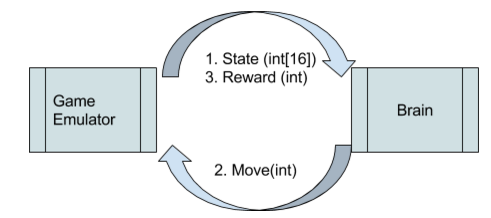
\includegraphics[width=60mm]{rl_state.png}

\end{centering}

We use a framework based on Torch 7 called DeepQLearning [9] to implement this process. The DeepQLearning framework provides the following Q-learning interface:

\begin{itemize}

\item \texttt{Brain.init(num\_inputs, num\_outputs)}: initialize the brain

\item \texttt{action = Brain.forward(state)}: generate movement based on game state

\item \texttt{Brain.backward(reward)}: train the neural network based on reward

\end{itemize}

In addition, the framework provides entry points to further configure the \texttt{Brain}. Here we provide our customization of 2048 puzzle game "brain":

\begin{itemize}

\item \texttt{Brain.temporal\_window = 0}. Due to instantaneous randomization, we take no past state/action pairs
\item \texttt{Brain.experience\_size = 10000}. Maximum number of experiences that we will save for training; this results in a maximum of 20 MB of storage. Further training experiences replace old ones.
\item \texttt{Brain.gamma = 0.99}. Decay factor which controls how much plan-ahead the agent does. Our choice leads to a factor of 0.36 after every 100 moves (number of moves for a game)
\item \texttt{Brain.epsilon = 1.0, Brain.epsilon\_min = 0.05}. Purely randomized to highly deterministic policy at end

\end{itemize}

Our reward function is \begin{align*}
\text{reward} =
\begin{cases}
100000000 & \text{if game is won} \\
100000000 & \text{if new highest tile found} \\
-\texttt{avg\_score} & \text{if game is lost} \\
\end{cases}
\end{align*}

Based on former strategies, a randomized agent has average performance of 571 points, with maximum 1456. By applying the reinforcement learning, our agent quickly surpasses this benchmark and begins generating scores up to 1000 frequently.

Around 5 minutes after training begins on a modern laptop, the agent is able to find the 128 tile in most simulations. Around 12 to 20 minutes after training, an interesting pattern can be observed: \textbf{the agent starts clustering large tiles together}.

The performance of reinforcement learning stabilizes at an average of 1200 points (highest 4548) after 2 hours of training.

\begin{centering}

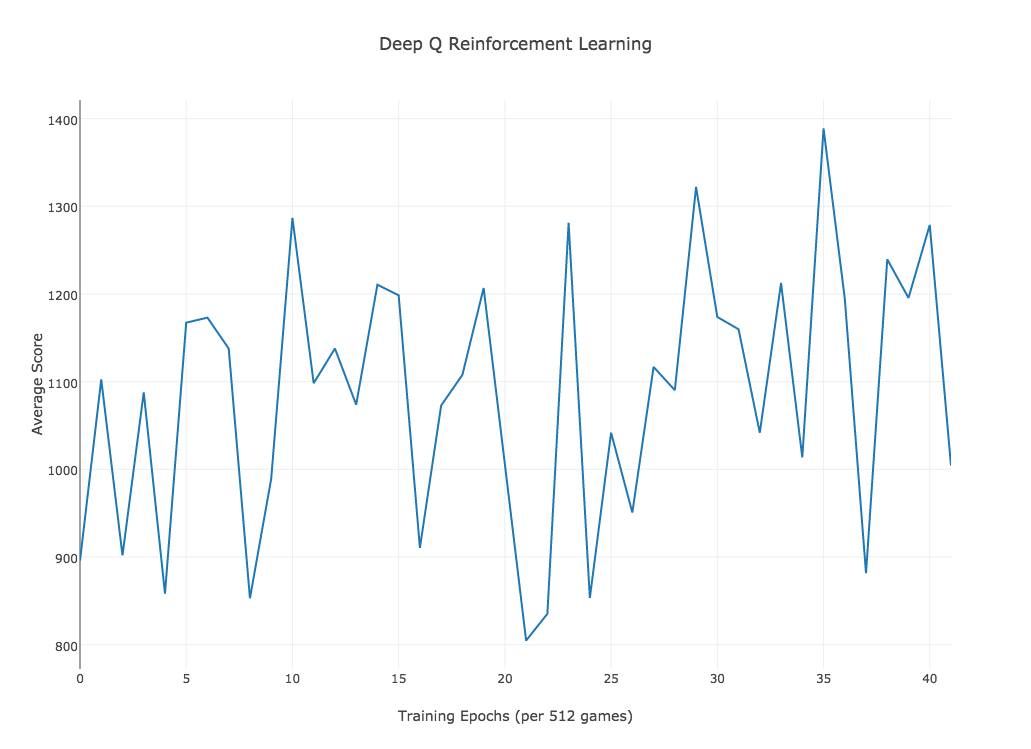
\includegraphics[width=60mm]{rl_graph.jpg}

\end{centering}

\section{Error Analysis and Future Works}

\subsection{Evaluation Functions}

Though the goal of this project was not to find the ideal evaluation function for 2048, we saw how critical a good evaluation function was to yielding good performance. In this project, we experimented with several different evaluation functions for the expectimax agent, and the “snake” evaluation function was able to give us the best success.

However, we do believe that the monotonicity, smoothness, empty tiles, and the raw score evaluation functions can be beneficial. Though we tried using a weighted combination of all five evaluation functions, with the hyperparameters we tried, the variance in total scores was greatly increased and the mean score was only sometimes marginally increased. However, to better tune the evaluation function, in the future, we can potentially better tune these hyperparameters for a combined evaluation function using a “parameter sweep” methodology. Additionally, we can explore other evaluation functions based on deeper domain knowledge.

\subsection{Machine Learning}

The performance of the reflex agents was far worse than expected. We can see several areas for improvement:

\begin{enumerate}[1)]

\item The dataset used to train the reflex agents was likely very biased. Specifically, we used several playthroughs of 2048 using the expectimax agent, saving every single board state and its corresponding recommended move. However, later in the game, larger-valued tiles or tiles which are “locked in” tend to stay in the same position for hundreds of moves. For instance, considering that the evaluation function tends to put the largest tile in the top left square, there tend to be two times as many data points containing a largest tile of value n than data points containing a largest tile of value $\frac{n}{2}$. Therefore, we hypothesize that such tiles repeatedly used in the training set failed to allow the reflex models to generalize. This was especially true in practice, since the vast majority of data points were from late in the game, while the reflex agent always failed early on.

\item Our models also likely had high bias. As demonstrated by our results, the process of picking moves in 2048 is clearly nonlinear, which explains the failure of single-layer models to generalize the move-making process. Furthermore, data from the expectimax agent with depth 3 likely had much deeper “strategy” than could be modelled by such small networks. (For instance, our team members noticed many signs of deeper “thinking” in the depth 3 agent as compared to even the depth 2 agent.) Therefore, to address the failure of our neural networks with one hidden layer to generalize the move-making process, we could look into larger and more advanced models, as well as explore different techniques.

\item Rather than simply unrolling the board into a vector in $\mathbb{R}^{16}$ and expecting our models to learn the underlying patterns to the moves, we could try using more descriptive features as inputs. For instance, we could take inspiration from our monotonicity, smoothness, and num-empty evaluation functions and use those as features to give our models more insight into the actual game state, rather than simply giving the raw tile values.

\item Instead of deterministically choosing the move with the highest output, we could easily implement an agent to randomly pick a move weighted by the outputs. This would be a simple way to avoid the problem of the models repeatedly picking the same move deterministically.

\end{enumerate}

\subsection{Reinforcement Learning}

Even though the reinforcement learning agent achieved high scores that can never be obtained by randomized movements, the average performance is still low compared to our expectimax agent. We think that this is partly due to the randomized nature of 2048. Because random tiles are created at every move, the game variability is much bigger than Atari, or other similar puzzles. Our dataset (2000 games) is hardly representative of the vast possibilities.

On the other hand, compared to the large game state space, there exists only one right way of solving the puzzle (lining up values in a snake-like fashion). It is very hard for reinforcement learning algorithms to find this approach simply based on randomized exploration. Even if it happens to achieve a high score in one game, the effect is averaged out by large number of low-score, low-reward game experiments.

For possible future work, we think that better reward function should be invented. The most fitting reward function should be able to filter out the few “correct” movements out of large number of randomized trials.

\begin{thebibliography}{9}

\bibitem{1} \texttt{https://github.com/ov3y/2048-AI}

\bibitem{2} Jason Lewis, Alec Powell, Jai Sajnani. "2048: An AI Agent".

\bibitem{3} Hadi Pouransari and Saman Ghili. "AI algorithms for the game 2048".

\bibitem{4} Prithvi Ramakrishnan. "Solving 2048".

\bibitem{5} \texttt{http://www.nature.com/nature/journal/\\v518/n7540/full/nature14236.html}

\bibitem{6} \texttt{http://flask.pocoo.org/}

\bibitem{7} \texttt{http://torch.ch/}

\bibitem{8} \texttt{https://en.wikipedia.org/wiki/Softmax\_function}

\bibitem{9} \texttt{https://github.com/blakeMilner/DeepQLearning}


\end{thebibliography}

\end{document}